\chapter{Arhitektura i dizajn sustava}

		Arhitektura se može podijeliti na tri podsustava:
		\begin{itemize}
			\item 	Web poslužitelj
			\item 	Web aplikacija
			\item 	Baza podataka		
		\end{itemize}

		\underbar{Web preglednik} predstavlja program koji omogućuje korisnicima 
		pregledavanje web-stranica i konzumiranje povezanih multimedijskih sadržaja. 
		Svaki internetski preglednik djeluje kao prevoditelj, interpretirajući kôd web 
		stranica napisan u određenom programskom jeziku i pretvarajući ga u vizualni 
		format razumljiv svakom korisniku. Drugim riječima, stranice su izvorno napisane 
		u kodu, a \textit{web preglednik} ih interpretira kako bi korisnicima pružio čitljiv i 
		interaktivan prikaz. Kada korisnik želi pristupiti određenoj web stranici, 
		šalje zahtjev \textit{web poslužitelju} putem \textit{web preglednika}, što pokreće proces 
		prijenosa informacija i omogućava korisnicima interakciju s odabranim sadržajem.


		\underbar{Web poslužitelj} zadužen je za komunikaciju
		klijenta sa aplikacijom. Međusobna komunikacija odvija se putem HTTP (engl. \textit{Hyper
		Text Transfer Protocol}) protokola, koji je jedan od protokola za prijenos informacija
		na webu.

		Korisnik koristi \textit{web aplikaciju} za obrađivanje željenih zahtjeva.
		\textit{Web aplikacija} gleda zahtjev te ovisno o njemu, pristupa bazi podataka nakon čega
		preko \textit{web poslužitelja} vraća korisniku odgovor u HTML dokumentu koji je 
		vidljiv u \textit{web pregledniku}.

		Programski jezik koji smo odabrali za izradu naše \textit{web aplikacije} je Java, zajedno
		sa Spring Boot radnim okvirom te programski jezik JavaScript zajedno sa React radnim okvirom.

		Ovisno o ulogama u timu, odabrana razvoja okruženja su:

		\begin{itemize}
			\item Frontend - Visual Studio Code
			\item Backend - Intellij IDEA
			\item Dokumentacija - Visual Studio Code		
		\end{itemize}

		Arhitekura sustava zasnivat će se na arh. obrascu MVC (Model-View-Controller).
		Spring Boot nudi veliku podršku za rad sa Spring MVC-om te kao takav
		odgovara našim zahtjevima (također olakšava konfiguraciju potrebnu za validan rad
		Spring MVC-a).

		Arh. obrazac MVC omogućava nezavisan razvoj pojedinih dijelova aplikacije te kao takav
		olakšava ispitivanje, razvijanje i dodavanje novih svojstva u aplikaciju.

		\medbreak

		Temeljne komponente MVC koncepta su:
		\begin{itemize}
			\item Model - dinamičke strukture podataka, npr. entitet User, Ingredient...
			\item View - ono što korisnik vidi, vizualizacija podataka
			\item Controller - poveznica između Model-a i View-a, bavi se HTTP zahtjevima i odgovorima		
		\end{itemize}

		\eject
				
		\section{Baza podataka}

			U našem sustavu, koristit ćemo relaciju bazu podataka koja je strukturom prilagođena
			modeliranju stvarnog svijeta. Osnovna gradivna jedinka baze je relacija, tj. tablica
			koja je identificirana svojim imenom i skupom atributa. Glavna svrha baze podataka je
			brza i jednostavna pohrana, izmjena te dohvat podataka za određenu uporabu.

			\medbreak

			Upravitelj bazom podataka:
			\begin{itemize}
				\item PostgreSQL		
			\end{itemize}

			\medbreak

			Entiteti baze podataka:
			\begin{itemize}
				\item users
				\item userFollow		
				\item chatMessage		
				\item communicationTime
				\item recipe		
				\item recipeRating		
				\item bookmarkedRecipe		
				\item role		
				\item category		
				\item tag		
				\item ingredient		
				\item cuisine		
				\item video		
				\item image		
				\item media				
			\end{itemize}
			
			\eject

			\subsection{Opis tablica}

				Relacija \textbf{users} pohranjuje entitete modela koji predstavlaju korisnika.
				Ograničenje stranog ključa odnosi se na atribut roleId koji označava id
				razine pristup (Klijent, Vlasnik, Admin) koju korisnik ima; referencirana je
				relacija role, stupac id. 
				
				\begin{longtblr}[
					label=none,
					entry=none
					]{
						width = \textwidth,
						colspec={|X[6,l]|X[6, l]|X[20, l]|}, 
						rowhead = 1,
					} %definicija širine tablice, širine stupaca, poravnanje i broja redaka naslova tablice
					\hline \SetCell[c=3]{c}{\textbf{users}}	 \\ \hline[3pt]
					\SetCell{LightGreen}id & INT	&  	jedinstveni identifikator korisnika  	\\ \hline
					firstName	& VARCHAR &   ime korisnika	\\ \hline 
					lastName & VARCHAR & prezime korisnika  \\ \hline 
					username & VARCHAR	&  korisničko ime korisnika		\\ \hline
					email & VARCHAR	&  adresa elektroničke pošte korisnika		\\ \hline
					password & VARCHAR	&  hash lozinke		\\ \hline 
					\SetCell{LightBlue} roleId	& VARCHAR &  identifikator razine pristupa korisnika (role.id) 	\\ \hline 
				\end{longtblr}

				Relacija \textbf{userFollow} pohranjuje entitete modela koji predstavlja odnos praćenja
				korisnika i autora.
				Ograničenje stranog ključa odnosi se na atribute followerId i authorId koji označavaju
				id korisnika koji je inicirao praćenje, tj. korisnika koji je autor recepta; referencirana je
				relacija users, stupac id.

				\begin{longtblr}[
					label=none,
					entry=none
					]{
						width = \textwidth,
						colspec={|X[6,l]|X[6, l]|X[20, l]|}, 
						rowhead = 1,
					} %definicija širine tablice, širine stupaca, poravnanje i broja redaka naslova tablice
					\hline \SetCell[c=3]{c}{\textbf{userFollow}}	 \\ \hline[3pt]
					\SetCell{LightGreen}id & INT	&  	jedinstveni identifikator modela praćenja	\\ \hline
					\SetCell{LightBlue} followerId	& INT &   id korisnika koji prati 	(user.id)\\ \hline 
					\SetCell{LightBlue} authorId & INT & id autora kojeg se prati  (user.id)\\ \hline 
					followedAt & TIMESTAMP	&  vrijeme početka praćenja		\\ \hline
				\end{longtblr}

				Relacija \textbf{chatMessage} pohranjuje entitete modela koji predstavlja
				poruke koje se koriste pri komunikaciji.
				Ograničenje stranog ključa odnosi se na atribute senderId i receiverId koji označavaju
				id korisnika koji je posalo poruku, tj. korisnika koji poruku treba primiti; referencirana je
				relacija users, stupac id.
				
				\begin{longtblr}[
					label=none,
					entry=none
					]{
						width = \textwidth,
						colspec={|X[6,l]|X[6, l]|X[20, l]|}, 
						rowhead = 1,
					} %definicija širine tablice, širine stupaca, poravnanje i broja redaka naslova tablice
					\hline \SetCell[c=3]{c}{\textbf{chatMessage}}	 \\ \hline[3pt]
					\SetCell{LightGreen}id & INT	&  	jedinstveni identifikator poruke (user.id)	\\ \hline
					\SetCell{LightBlue} senderId	& INT &  id pošiljatelja (user.id)  	\\ \hline 
					\SetCell{LightBlue} receiverId & INT & id primatelja (user.id) \\ \hline 
					content & VARCHAR	&  sadržaj poruke		\\ \hline
				\end{longtblr}

				Relacija \textbf{communicationTime} pohranjuje entitete modela koji predstavlja
				dostupnost korisnika za komunikaciju.
				Ograničenje stranog ključa odnosi se na atribut userId koji označava
				id korisnika koji prikazuje vrijeme u koje je dostupan za komunikaciju; referencirana je
				relacija users, stupac id.

				\begin{longtblr}[
					label=none,
					entry=none
					]{
						width = \textwidth,
						colspec={|X[6,l]|X[6, l]|X[20, l]|}, 
						rowhead = 1,
					} %definicija širine tablice, širine stupaca, poravnanje i broja redaka naslova tablice
					\hline \SetCell[c=3]{c}{\textbf{communicationTime}}	 \\ \hline[3pt]
					\SetCell{LightGreen}id & INT	&  	jedinstveni identifikator \\ \hline
					\SetCell{LightBlue}userId	& INT &   jedinstveni identifikator korisnika (user.id)\\ \hline 
					\SetCell{LightBlue}start & TIMESTAMP & vrijeme od  \\ \hline 
					\SetCell{LightBlue}end & TIMESTAMP	&  vrijeme do		\\ \hline
				\end{longtblr}

				Relacija \textbf{recipe} pohranjuje entitete modela recept.
				Ograničenje stranog ključa odnosi se na atribute ingredientId, tagId, categoryId, cuisineId, mediaId
				te userId koji označavaju, redom, sastojke recepta, oznake recepta, kategoriju u koju recept spada,
				kuhinju u koju recept spada, multimedijske sadržaje koje recept sadrži te autora recepta.
				Relacije koje se referenciraju su, redom, ingredient (stupac id), tag (stupac id), category (stupac id),
				cuisine (stupac id), media (stupac id), user (stupac id). 
				
				Zbog jednostavnosti vizualnog prikaza, odnosi @ManyToMany nisu prikazani zasebnom relacijom.
				
				Redom:
				\begin{itemize}
					\item 	N:N sa ingredient
					\item 	N:N sa tag
					\item 	N:N sa media	
				\end{itemize}

				\begin{longtblr}[
					label=none,
					entry=none
					]{
						width = \textwidth,
						colspec={|X[6,l]|X[6, l]|X[20, l]|}, 
						rowhead = 1,
					} %definicija širine tablice, širine stupaca, poravnanje i broja redaka naslova tablice
					\hline \SetCell[c=3]{c}{\textbf{recipe}}	 \\ \hline[3pt]
					\SetCell{LightGreen}id & INT	&  	jedinstveni identifikator recepta  	\\ \hline
					\SetCell{LightBlue} ingredientId	& List<INT> &   id sastojka 	(ingredient.id)\\ \hline 
					\SetCell{LightBlue} tagId	& INT &   id oznake	(tag.id)\\ \hline 
					\SetCell{LightBlue} categoryId	& INT &   id kategorije	(category.id)\\ \hline 
					\SetCell{LightBlue} cuisineId & INT & id zemlje podrijetla (cuisine.id) \\ \hline 
					\SetCell{LightBlue} mediaId & INT & id multimedijske stavke (media.id) \\ \hline 
					\SetCell{LightBlue} userId & INT	&  id autora (user.id)	\\ \hline
					title & VARCHAR	&  naslov recepta		\\ \hline
					description & VARCHAR	& opis recepta		\\ \hline 
					cookingTime	& INTERVAL &  vrijeme kuhanja 	\\ \hline 
				\end{longtblr}

				Relacija \textbf{recipeRating} pohranjuje modele entiteta koji predstavljaju
				\textit{feedback} na recept; ocjenu i komentar.
				Ograničenje stranog ključa odnosi se na atribute userId i recipeId koji označavaju
				id korisnika koji daje \textit{feedback} i recept koji se komentira; referencirana je
				relacija users, stupac id te relacija recipe, stupac id.

				\begin{longtblr}[
					label=none,
					entry=none
					]{
						width = \textwidth,
						colspec={|X[6,l]|X[6, l]|X[20, l]|}, 
						rowhead = 1,
					} %definicija širine tablice, širine stupaca, poravnanje i broja redaka naslova tablice
					\hline \SetCell[c=3]{c}{\textbf{recipeRating}}	 \\ \hline[3pt]
					\SetCell{LightGreen}id & INT	&  	jedinstveni identifikator ocjene  	\\ \hline
					\SetCell{LightBlue} userId & INT	&  id klijenta koji je dao ocjenu (user.id)	\\ \hline 
					\SetCell{LightBlue} recipeId & INT & id recepta (recipe.id) \\ \hline 
					rating& INT	&  ocjena	\\ \hline
					comment & VARCHAR	&  komentar		\\ \hline
					createdAt & TIMESTAMP	& vrijeme nastanka ocjene		\\ \hline  
				\end{longtblr}

				Relacija \textbf{bookmarkedRecipe} pohranjuje model entiteta koji predstavlja zabilježbu recepta
				od strane nekog korisnika.
				Ograničenje stranog ključa odnosi se na atribute userId i recipeId koji označavaju
				id korisnika koji zabilježuje recept te id recepta koji se zabilježuje; referencirana je
				relacija users, stupac id te relacija recipe, stupac id.

				\begin{longtblr}[
					label=none,
					entry=none
					]{
						width = \textwidth,
						colspec={|X[6,l]|X[6, l]|X[20, l]|}, 
						rowhead = 1,
					} %definicija širine tablice, širine stupaca, poravnanje i broja redaka naslova tablice
					\hline \SetCell[c=3]{c}{\textbf{bookmarkedRecipe}}	 \\ \hline[3pt]
					\SetCell{LightGreen}id & INT	&  	jedinstveni identifikator zabilježbe recepta  	\\ \hline
					\SetCell{LightBlue} userId & INT	&  id klijenta koji je dao ocjenu (user.id)	\\ \hline 
					\SetCell{LightBlue} recipeId & INT & id recepta (recipe.id) \\ \hline 
					createdAt & TIMESTAMP	& vrijeme nastanka ocjene		\\ \hline  
				\end{longtblr}

				\textbf{role} Relacija pohranjuje model entiteta koji predstavlja
				"ulogu", tj. razinu prava pristupa korisnika (Klijent, Vlasnik, Autor).

				\begin{longtblr}[
					label=none,
					entry=none
					]{
						width = \textwidth,
						colspec={|X[6,l]|X[6, l]|X[20, l]|}, 
						rowhead = 1,
					} %definicija širine tablice, širine stupaca, poravnanje i broja redaka naslova tablice
					\hline \SetCell[c=3]{c}{\textbf{role}}	 \\ \hline[3pt]
					\SetCell{LightGreen}id & INT	&  	jedinstveni identifikator razine pristupa\\ \hline
					name	& VARCHAR &  ime razine pristupa  	\\ \hline 
				\end{longtblr}

				Relacija \textbf{category} pohranjuje model entiteta koji predstavlja
				kategoriju u koju recept može pripadati.

				\begin{longtblr}[
					label=none,
					entry=none
					]{
						width = \textwidth,
						colspec={|X[6,l]|X[6, l]|X[20, l]|}, 
						rowhead = 1,
					} %definicija širine tablice, širine stupaca, poravnanje i broja redaka naslova tablice
					\hline \SetCell[c=3]{c}{\textbf{category}}	 \\ \hline[3pt]
					\SetCell{LightGreen}id & INT	&  	jedinstveni identifikator kategorije\\ \hline
					name	& VARCHAR &  ime kategorije  	\\ \hline 
				\end{longtblr}

				Relacija \textbf{tag} pohranjuje model entiteta koji predstavlja
				oznaku koji recept može imati (npr. Vegan, Healthy, Quick...)
				
				\begin{longtblr}[
					label=none,
					entry=none
					]{
						width = \textwidth,
						colspec={|X[6,l]|X[6, l]|X[20, l]|}, 
						rowhead = 1,
					} %definicija širine tablice, širine stupaca, poravnanje i broja redaka naslova tablice
					\hline \SetCell[c=3]{c}{\textbf{tag}}	 \\ \hline[3pt]
					\SetCell{LightGreen}id & INT	&  	jedinstveni identifikator oznake recepta\\ \hline
					name	& VARCHAR &  opis oznake recepta  	\\ \hline 
				\end{longtblr}

				Relacija \textbf{ingredient} pohranjuje model entiteta koji predstavlja
				sastojak koji recept može sadržavati.

				\begin{longtblr}[
					label=none,
					entry=none
					]{
						width = \textwidth,
						colspec={|X[6,l]|X[6, l]|X[20, l]|}, 
						rowhead = 1,
					} %definicija širine tablice, širine stupaca, poravnanje i broja redaka naslova tablice
					\hline \SetCell[c=3]{c}{\textbf{ingredient}}	 \\ \hline[3pt]
					\SetCell{LightGreen}id & INT	&  	jedinstveni identifikator sastojka\\ \hline
					name	& VARCHAR &  ime sastojka  	\\ \hline 
				\end{longtblr}

				\textbf{cuisine} Relacija pohranjuje model entiteta koji predstavlja
				zemlju podrijetla recepta, tj. kuhinju iz koje recept potječe.

				\begin{longtblr}[
					label=none,
					entry=none
					]{
						width = \textwidth,
						colspec={|X[6,l]|X[6, l]|X[20, l]|}, 
						rowhead = 1,
					} %definicija širine tablice, širine stupaca, poravnanje i broja redaka naslova tablice
					\hline \SetCell[c=3]{c}{\textbf{cuisine}}	 \\ \hline[3pt]
					\SetCell{LightGreen}id & INT	&  	jedinstveni identifikator zemlje kuhanja\\ \hline
					name	& VARCHAR &  ime zemlje kuhanja  	\\ \hline 
				\end{longtblr}

				Relacija \textbf{video} pohranjuje model entiteta koji predstavlja
				medijski zapis oblika videa.

				\begin{longtblr}[
					label=none,
					entry=none
					]{
						width = \textwidth,
						colspec={|X[6,l]|X[6, l]|X[20, l]|}, 
						rowhead = 1,
					} %definicija širine tablice, širine stupaca, poravnanje i broja redaka naslova tablice
					\hline \SetCell[c=3]{c}{\textbf{video}}	 \\ \hline[3pt]
					\SetCell{LightGreen}id & INT	&  	jedinstveni identifikator videa\\ \hline
					duration	& INTERVAL &  trajanje videa  	\\ \hline 
				\end{longtblr}

				\textbf{image} Reliacija pohranjuje model entiteta koji predstavlja
				medijski zapis oblika fotografije.

				\begin{longtblr}[
					label=none,
					entry=none
					]{
						width = \textwidth,
						colspec={|X[6,l]|X[6, l]|X[20, l]|}, 
						rowhead = 1,
					} %definicija širine tablice, širine stupaca, poravnanje i broja redaka naslova tablice
					\hline \SetCell[c=3]{c}{\textbf{image}}	 \\ \hline[3pt]
					\SetCell{LightGreen}id & INT	&  	jedinstveni identifikator fotografije\\ \hline
					width	& INT &  širina fotografije (px)  	\\ \hline
					height	& INT &  visina fotografije (px)  	\\ \hline
					format  & VARCHAR & format fotografije \\ \hline
				\end{longtblr}
				
				\eject

				Relacija \textbf{media} pohranjuje model entiteta koji predstavlja medijski sadržaj
				koji je objavio neki korisnik, uz neki recept.
				Ograničenje stranog ključa odnosi se na atribute recipeId 
				id recepta uz okji je medijski sadržaj postavljen; referencirana je
				relacija recipe, stupac id.

				Medijska stavka može biti ili slika ili video.

				\begin{longtblr}[
					label=none,
					entry=none
					]{
						width = \textwidth,
						colspec={|X[6,l]|X[6, l]|X[20, l]|}, 
						rowhead = 1,
					} %definicija širine tablice, širine stupaca, poravnanje i broja redaka naslova tablice
					\hline \SetCell[c=3]{c}{\textbf{media}}	 \\ \hline[3pt]
					\SetCell{LightGreen}id & INT	&  	jedinstveni identifikator multimedijske stavke\\ \hline
					\SetCell{LightBlue}recipeId	& INT &  id recepta (px)  	\\ \hline
					key	& VARCHAR &   	naziv datoteke na oblaku\\ \hline
					description  & VARCHAR & opis multimedijske stavke \\ \hline
					uploadDate  & DATE & datum postavljanje multimedijske stavke \\ \hline

				\end{longtblr}
				
				\eject

				
				
			
			\subsection{Dijagram baze podataka}

			\begin{figure}[H]
				\rotatebox{90}{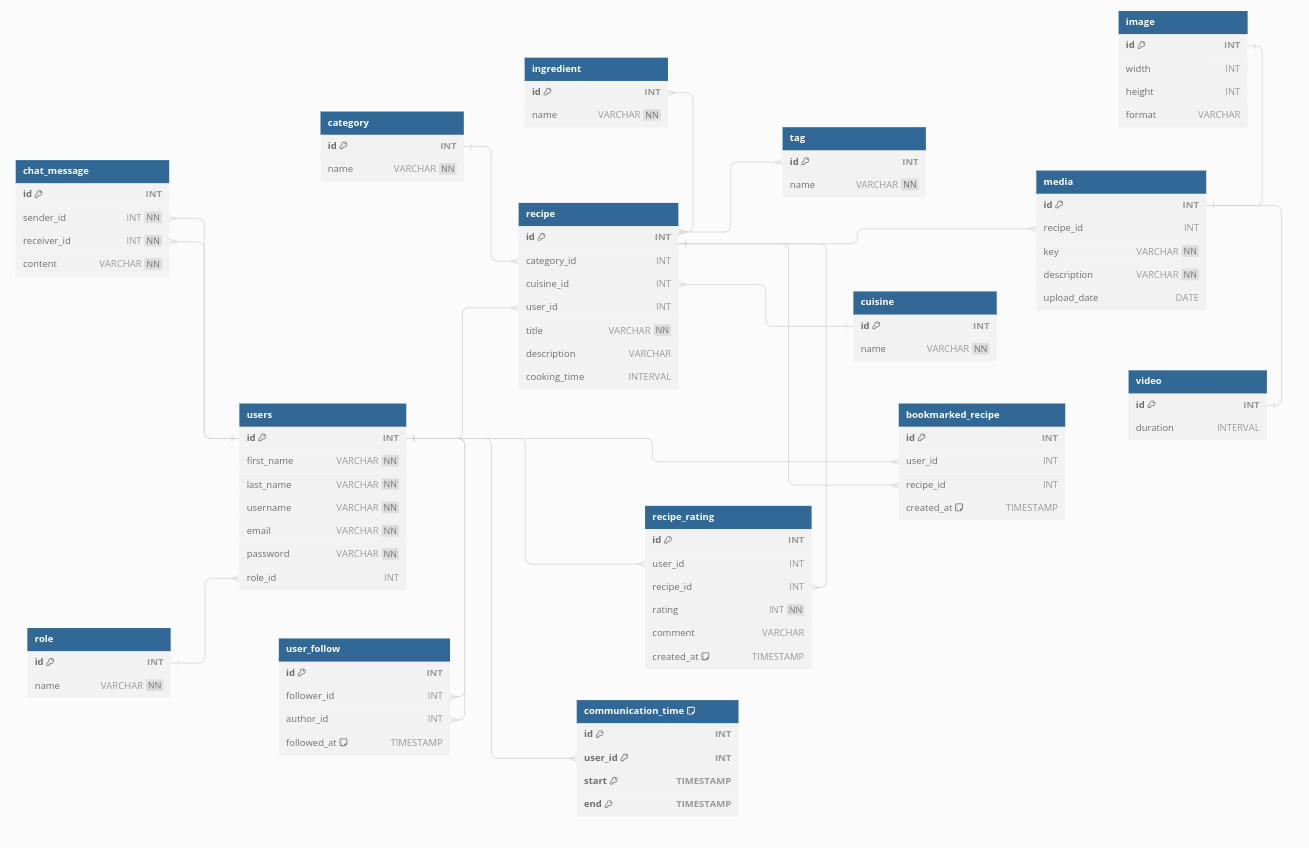
\includegraphics[scale=0.45]{dijagrami/dijagram_baze.png}} 
				\centering
				\caption{Dijagram baze podataka}
				\label{fig:bpdiag}
			\end{figure}
			
			
		\section{Dijagram razreda}

		Slike 4.2, 4.3 i 4.4 prikazuju razrede koji pripadaju backend dijelu odabrane
		arhitektura sustava (MVC). Razredi prikazani na slici 4.3 nasljeđuju Controller
		razred. Metode unutar tih razreda služe za manipulaciju podatcima pomoću
		DTO-a (Data Transfer Object). Podatci se dobivaju kroz metode koje su implementirane
		u Model razredima. Metode unutar Controller razreda odgovorne su za generiranje JSON datoteka
		i odgovarajućeg HTML statusnog koda kao povratne informacije na njihovo izvršavanje.

		\eject
		
		\begin{figure}[H]
			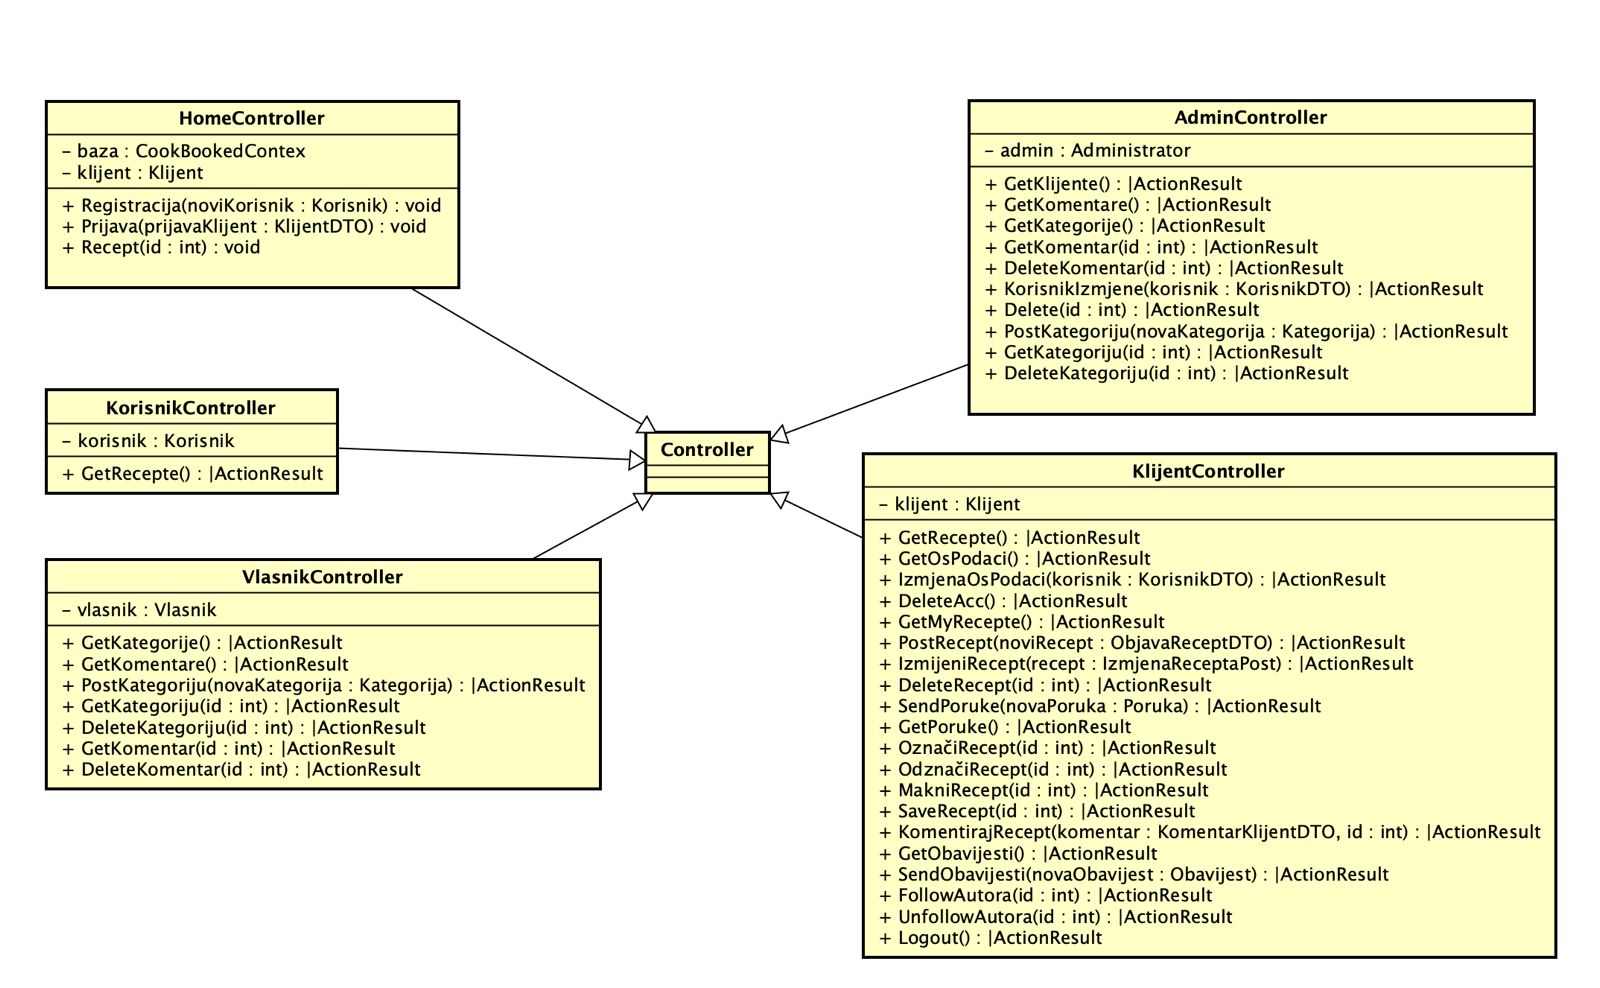
\includegraphics[scale=0.32]{dijagrami/razdijag_controller.jpeg} 
			\centering
			\caption{Dijagram razreda - dio Controllers}
			\label{fig:bpdiag}
		\end{figure}

		\eject

		\begin{figure}[H]
			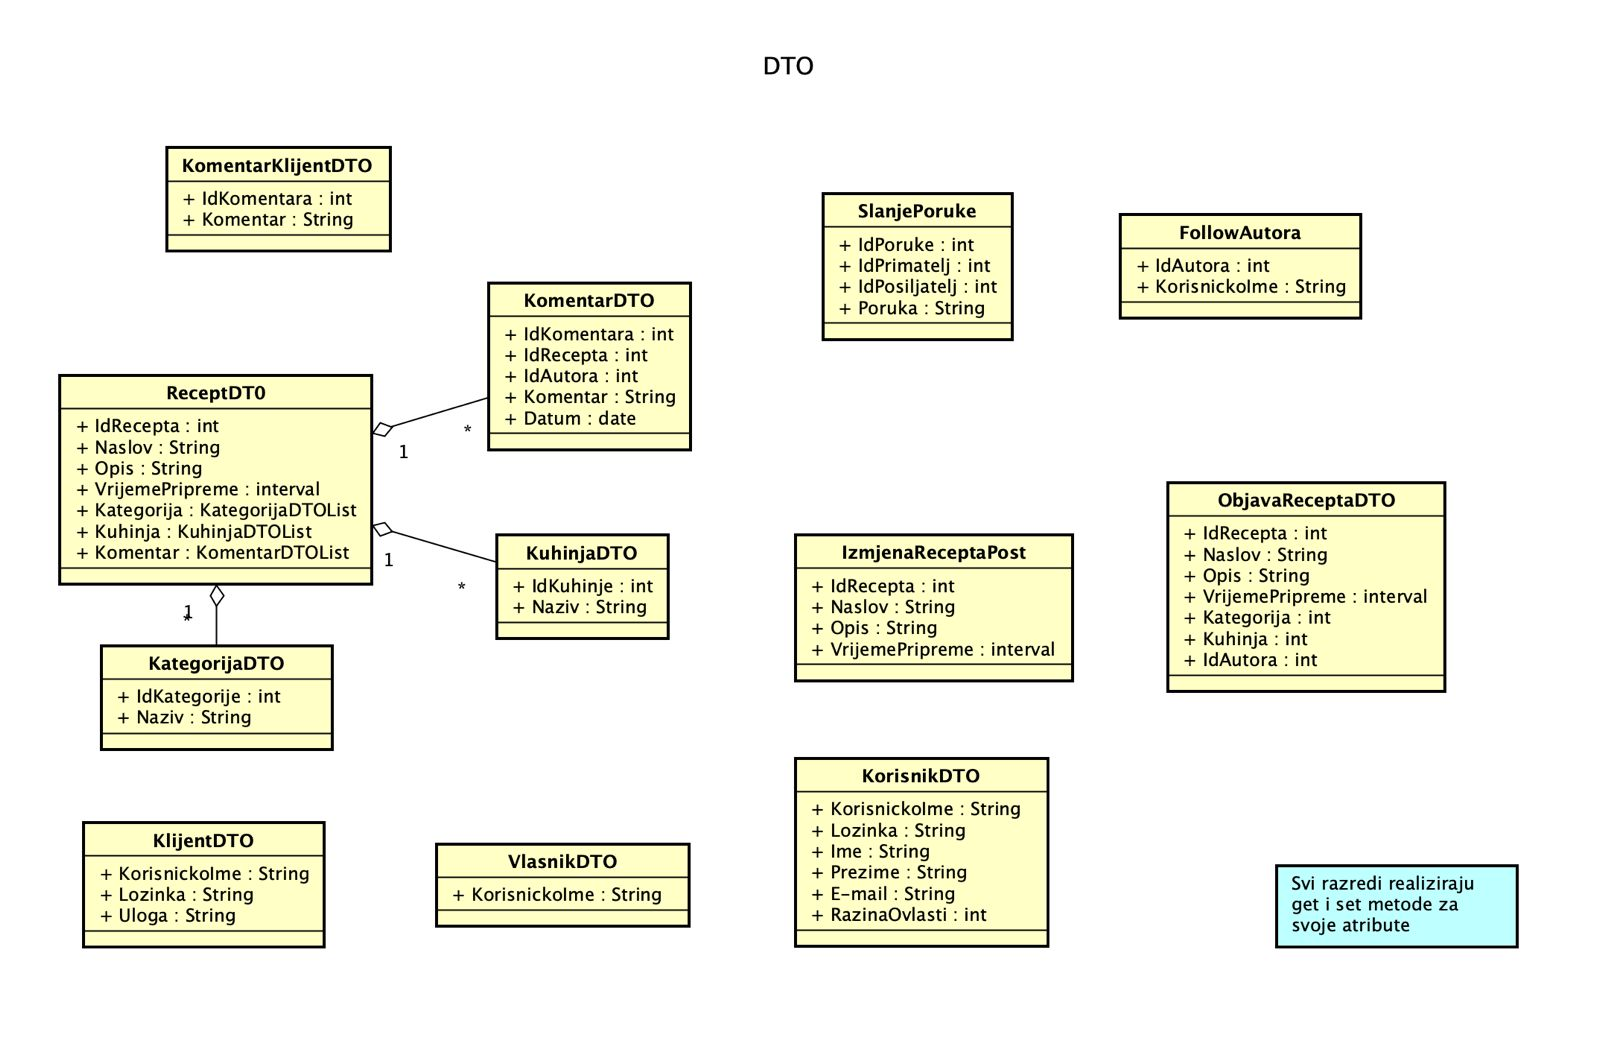
\includegraphics[scale=0.32]{dijagrami/razdijag_dto.jpeg}
			\centering
			\caption{Dijagram razreda - dio Data transfer objects}
			\label{fig:bpdiag}
		\end{figure}

		\eject

		\begin{figure}[H]
			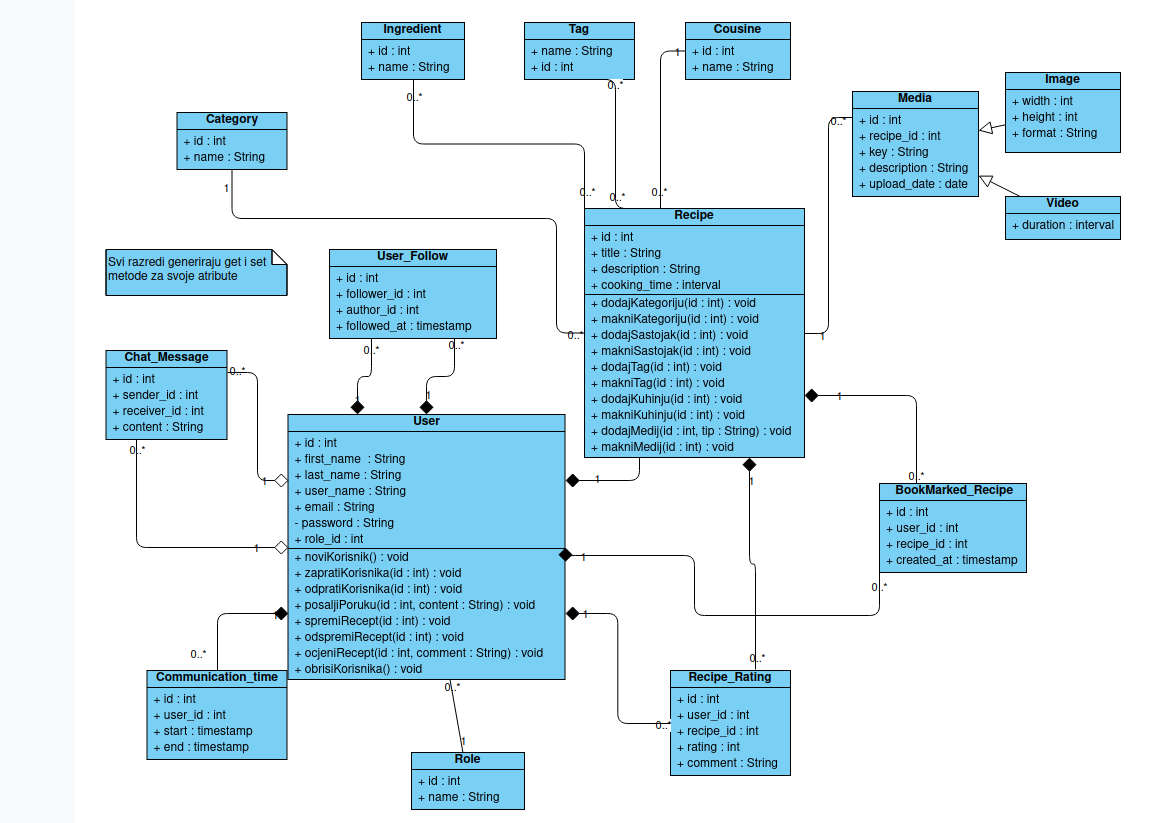
\includegraphics[scale=0.4]{dijagrami/razdijag_model.png}
			\centering
			\caption{Dijagram razreda - dio Models}
			\label{fig:bpdiag}
		\end{figure}

		\eject

		\section{Dijagrami nakon implementacije programskih rješenja}
		Prikaz dijagrama razreda nakon završetka druge faze projekta nalazi se direktoriju
		"/Dokumentacija" u dva oblika:

		\begin{itemize}
			\item 	CookBookedModel.plantuml
			\item 	CookBookedModelImage.png
		\end{itemize}

		Izvedba je u ovom obliku zbog preglednosti prikaza istih.

		Grafovi su automatski generirani pomoću IntelliJ IDEA Ultimate razvojnog okruženja.

		\eject

		\section{Dijagram stanja}
		Dijagram stanja prikazuje stanja objekata te prijelaze iz jednog stanja u drugo
		temeljene na događajima. Na slici 4.5 prikazan je dijagram stanja za registriranog
		korisnika.

		\noindent Nakon što se prijavi, klijent je preusmjeren na početnu stranicu s koje može
		pristupiti ostalim stranicama ("Postavke profila", "Moji recepti", "Dodavanje recepta", "Stranica s receptima",
		"Pregledavanje pristiglih poruka").

		\noindent Ako klijent odluči pregledavati recepte, iz padajućeg izbornika ima opciju
		filtrirati iste po kategoriji, kuhinji ili sastojcima recepta. Nakon prikaza svih filtriranih
		recepata, klijent može detaljnije pregledati svaki pojedinačni recept te objaviti komentar ili
		kontaktirati njegova autora.

		\noindent Preostale stranice nude očekivane opcije vezane uz postavke korisničkog profila,
		brisanje korisničkog profila, uređivanje već objavljenih recepata, njihovo brisanje, dodavanje novih
		te komunikaciju sa korisnicima koji sutemeljem već objavljenih recepata klijenta kontaktirali.

		\begin{figure}[H]
			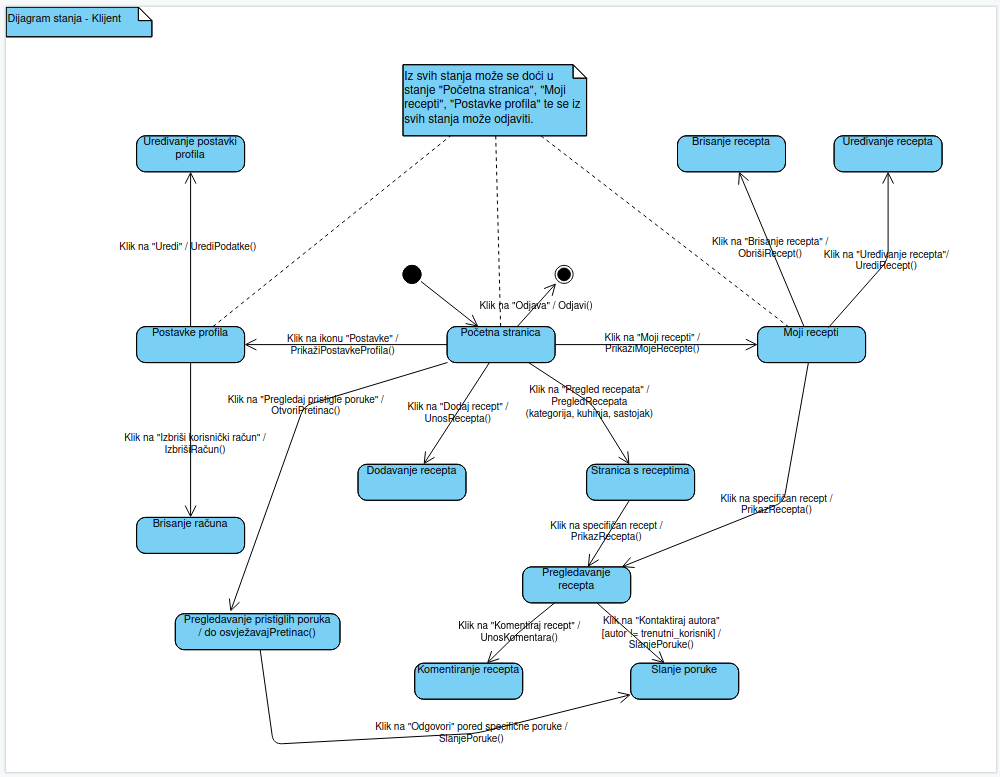
\includegraphics[scale=0.42]{dijagrami/dijagram_stanja.png}
			\centering
			\caption{Dijagram stanja}
			\label{fig:bpdiag}
		\end{figure}
		\eject
		
		\section{Dijagram aktivnosti}

		\noindent Na slici 4.6 prikazi su procesi akcija koje korisnik može izvršiti ukoliko se nađe na početnoj stranici.
		Detaljnije je obrađen slučaj ako korisnik želi pregledati pojedine recepte.
		Korisnik se prijavi u sustav, odabere koju stranicu želi vidjeti (detaljnije obrađena stranica prikaza recepata),
		a odabirom prikaza recepata prikažu mu se recepti. Odabirom pojedinog recepta korisnik može komentirati recept,
		poslati poruku autoru ili, ako je recept njegov, urediti podatke o receptu.

		\noindent Svaka od akcija uključuje ispunjenje određe forme od strane korisnika, slanje upita od strane web-aplikacije
		bazi podatakam potom odgovor baze podataka na taj upit te prikaz tog odgovora od strane web-aplikacije.

		\eject

		\begin{figure}[H]
			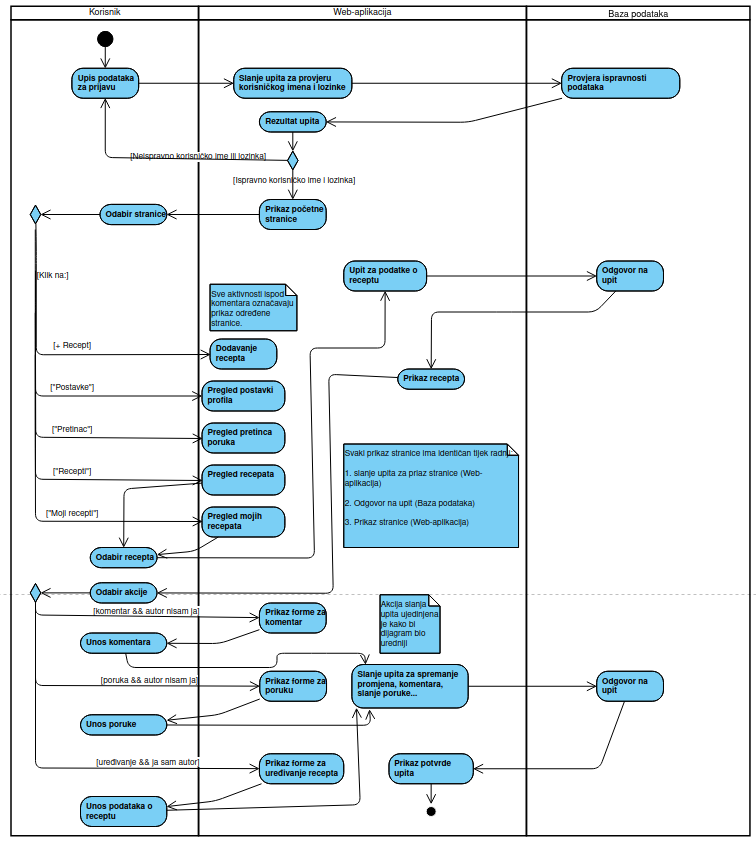
\includegraphics[scale=0.6]{dijagrami/dijagram_aktivnosti.png}
			\centering
			\caption{Dijagram aktivnosti}
			\label{fig:bpdiag}
		\end{figure}

		\eject

		\noindent Na slici 4.7 prikazan je dijagram komponenti koji opisuje organizaciju i međuovisnost
		komponenti, interne strukture i odnose prema okolini.

		\noindent Sustavu se može pristupiti preko dva raziličita sučelja:

		\medbreak
		\noindent 1. Sučelje za dohvat HTML, CSS i JS datoteka

		- služi za posluživanje datoteka koje pripadaju \textit{frontend} dijelu aplikacije

		- router je komponenta koja ovisno o url-u u upitu poslužuje određene datoteke
		
		- \textit{frontend} dio sastoji se od niza JavaScript datoteka raspoređenih u logičke 
		
		cjeline
		
		- JavaScript datoteke ovise o React biblioteci
		
		\medbreak
		\noindent 2. Sučelje za dohvat JSON podataka

		- preko njega se pristupa REST API komponenti
		
		- REST API poslužuje podatke koji pripadaju \textit{backend} dijelu aplikacije

		- Hibernate je zadužen za dohvaćanje tablica iz baze podataka pomoću SQL 
		
		upita

		- podaci koji su pristigli iz baze se šalju dalje MVC arhitekturi u obliku DTO-a 
		
		i/ili modela

		\medbreak
		\noindent React-view komponenta preko dosputnih sučelja komunicira sa CookBooked aplikacijom,
		omogućuje ažuriranje prikaza ovisno o korisničkim radnjama te omogućuje dohvaćanje novih podataka
		ili datoteka prema potrebi.

		\eject

		\begin{figure}[H]
			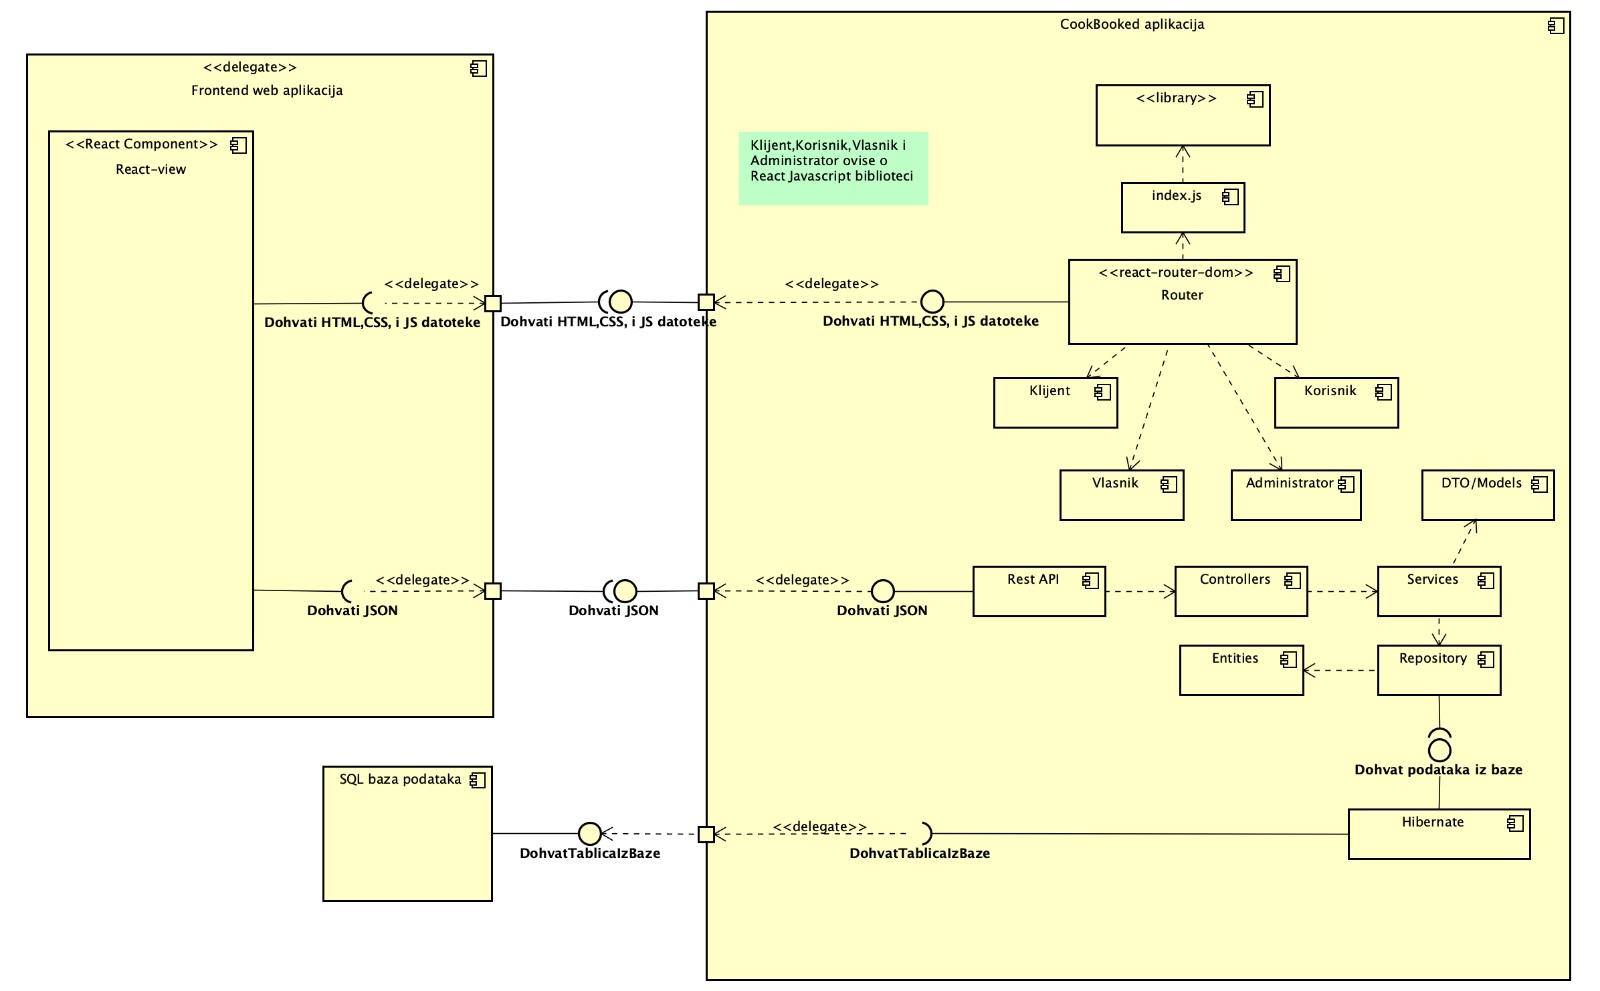
\includegraphics[scale=0.2]{dijagrami/dijagram_komponenti.jpeg}
			\centering
			\caption{Dijagram aktivnosti}
			\label{fig:bpdiag}
		\end{figure}
		\eject